\documentclass{beamer}
    \usetheme{Boadilla}
\usepackage{polyglossia}
    \setmainlanguage{german}
\usepackage{fontspec}
    \setsansfont{Linux Biolinum O}
\usepackage{graphicx}
\usepackage{xcolor}
\usepackage{listings}
    \lstset{language=bash,
	basicstyle=\footnotesize\ttfamily\tiny,
	breaklines=true,
	framextopmargin=50pt,
	frame=bottomline,
	backgroundcolor=\color{white!86!black},
	commentstyle=\color{blue},
	keywordstyle=\color{red},
	stringstyle=\color{orange!80!black}}
\usepackage{amsmath}
\usepackage{amssymb}
\usepackage{siunitx}
\usepackage{booktabs}
\usepackage{float}
\usepackage{tabularx}
\usepackage{caption}
\usepackage{subfig}
\usepackage{tikz}
\usepackage{hyperref}
     \hypersetup{
     colorlinks=true,
     linkcolor=black,
     filecolor=magenta}

\title{\texorpdfstring{\color{blue!50!black}\textbf{Status report - Thursday, April 30th}}{}}
\subtitle{Noise Occupancy Scans and Fake Hit rate}
\author{Maurice Donner}
\date{30. April 2020}

\begin{document}

\maketitle

% !TEX root = main.tex
% !TEX program = xelatex

\section{Übersicht}

\begin{frame}{Note to last Presentation}
    \begin{minipage}{.49\textwidth}
	\centering
	0 V Back Bias
    \begin{figure}[H]
	\centering
	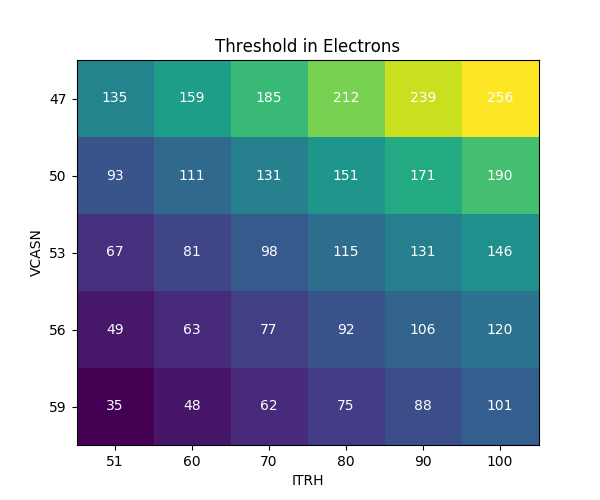
\includegraphics[width=\textwidth]{bb0_Heatmap_corrected.png}
    \end{figure}
    \raggedright
    \tiny
    Note: This is a corrected Version of the presentation. The Errors in
    data have been identified and fixed. The
    missing config file has been restored, and faulty values have been
    masked entirely. This is an accurate reference to all values.
    \end{minipage}
    \begin{minipage}{.49\textwidth}
	\centering
	3 V Back Bias
    \begin{figure}[H]
	\centering
	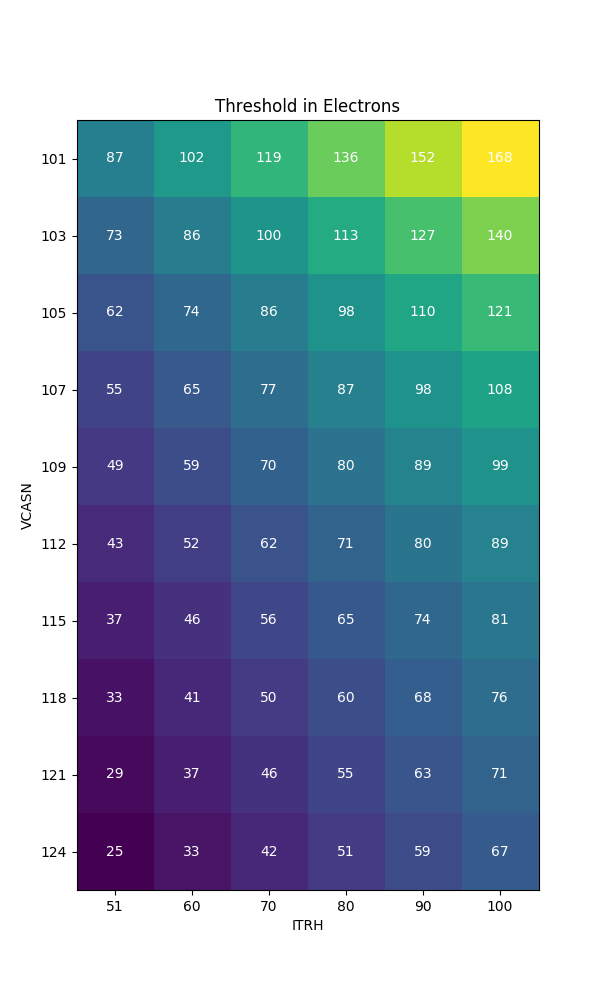
\includegraphics[width=0.75\textwidth]{bb3_Heatmap_corrected.png}
    \end{figure}
    \end{minipage}\\[.5cm]
\end{frame}

\begin{frame}[fragile]{Processing NoiseOcc Scan Data}
    \Large{Goals}\\
    \normalsize
    Automize the process of calculating Fake Hit Rate for any set of
    measurements\\
    \Large{Problems}\\
    \normalsize
    Pixel firings are completely random for the (well-working) pixels.\\
    -> no hit, no .dat file
    \pause
\begin{lstlisting}
MISSING=$(ls $PATHTOFILES | grep "NoiseOccupancy_$TIMESTAMP.dat")
if [[ "$MISSING" == "" ]]; then
    printf '%s\n' "$TIMESTAMP" "$VCASN" "$ITHR" "$SENLIM" "0" | paste -sd ',' >> output.csv
    echo "No hits registered, continuing"
else
    printf "Starting evaluation for run $TIMESTAMP with ITHR=$ITHR and VCASN=$VCASN \n"
    FHR=$(./FakeHit.py $DAT $NTRIGGERS | head -n 1)
    DFHR=$(./FakeHit.py $DAT $NTRIGGERS | tail -n 1)
$
\end{lstlisting}
\end{frame}

\begin{frame}[fragile]{Fake Hit rate}
    \begin{minipage}{.7\textwidth}
    \begin{figure}[H]
	\centering
	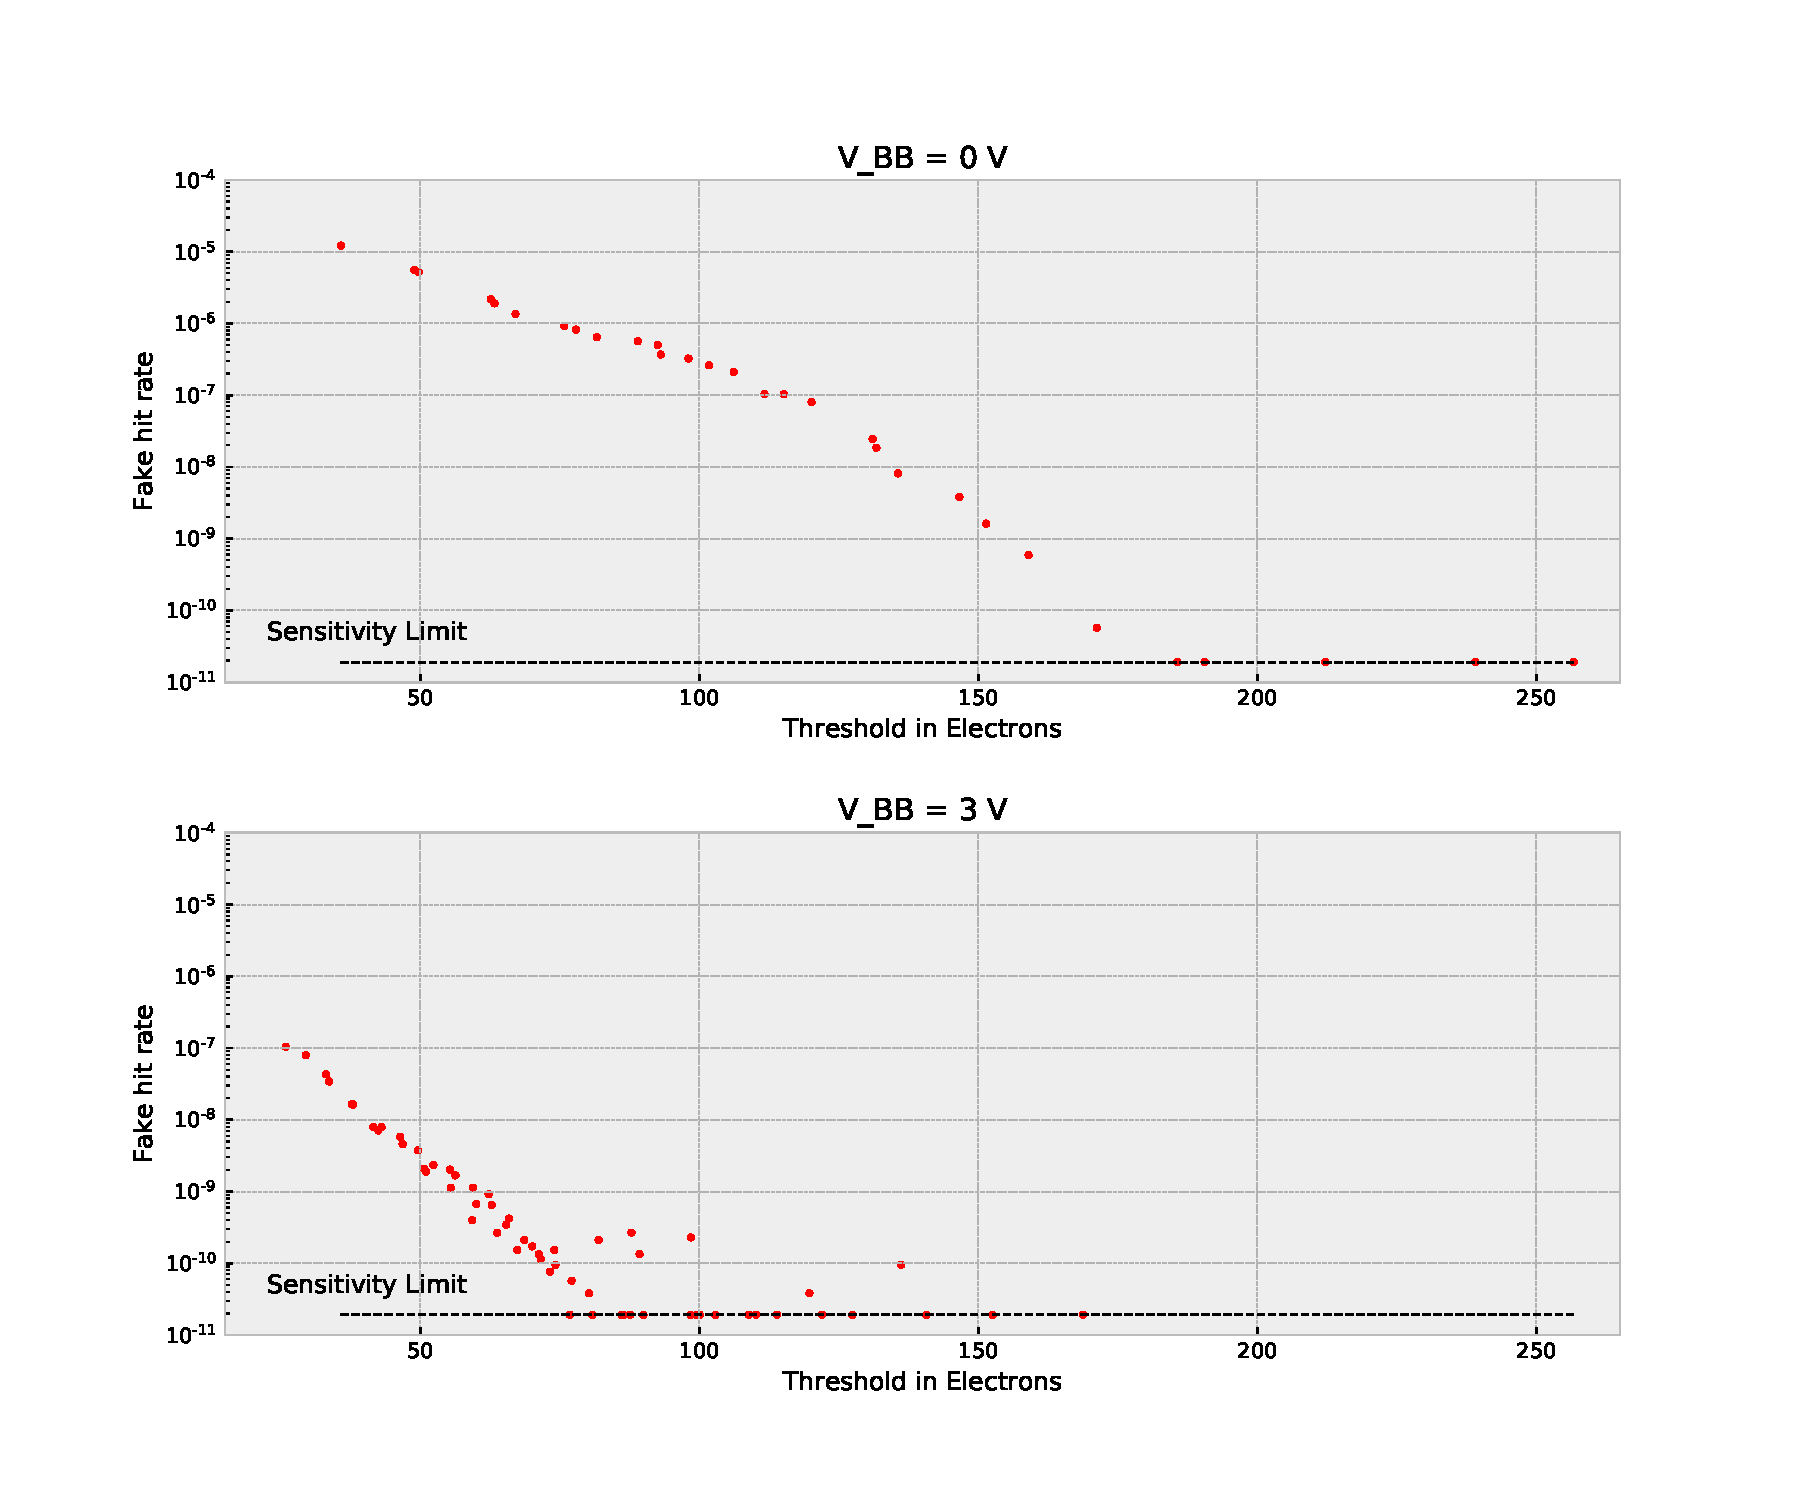
\includegraphics[width=\textwidth]{../Fake_Hit_Rate.pdf}
    \end{figure}
    \end{minipage}
    \pause
    \begin{minipage}{.29\textwidth}
	\tiny
	NoiseOccupancy\_200323\_185942.dat
\begin{lstlisting}
119 640 2
464 581 1
464 583 1
464 584 1
464 585 1
464 586 1
464 587 1
464 588 1
465 580 1
465 581 1
465 582 1
465 584 1
465 585 1
465 586 1
465 587 1
\end{lstlisting}
\begin{itemize}
    \item Cluster, induced by particle event during measurement
    \item random firing of column
\end{itemize}
    \end{minipage}
\end{frame}

\begin{frame}{New Stuff: Cosmics}
    \Large Goals \\
    \normalsize
    \begin{itemize}
	\item Take data over long periods of time automatically (so far there
	    are too many errors)
	    \pause
	\item Write scripts to search for cosmic events in huge data files.\\
	    \small Angular Distribution?
	    \pause
	\item \normalsize Analysis on Cosmics data
    \end{itemize}
\end{frame}


\end{document}
